\documentclass[12pt,utf8,notheorems,compress,t]{beamer}
\usepackage{etex}

\usepackage{pgfpages}
\usepackage[export]{adjustbox}

% Workaround for the issue described at
% https://tex.stackexchange.com/questions/164406/beamer-using-href-in-notes.
\newcommand{\fixedhref}[2]{\makebox[0pt][l]{\hspace*{\paperwidth}\href{#1}{#2}}\href{#1}{#2}}

\usepackage[english]{babel}

\usepackage[normalem]{ulem}
\usepackage{graphbox}
\usepackage{mathtools}
\usepackage{booktabs}
\usepackage{stmaryrd}
\usepackage{amssymb}
\usepackage{array}
\usepackage{ragged2e}
\usepackage{multicol}
\usepackage{tabto}
\usepackage{xstring}
\usepackage{proof}
\usepackage{ifthen}
\usepackage[normalem]{ulem}
\usepackage[all]{xy}
\xyoption{rotate}
\usepackage{tikz}
\usetikzlibrary{calc,shapes,shapes.callouts,shapes.arrows,patterns,fit,backgrounds,decorations.pathmorphing,positioning}
\hypersetup{colorlinks=true}

\newcommand*\circled[1]{\tikz[baseline=(char.base)]{%
  \node[shape=circle,draw,inner sep=1pt] (char) {#1};}}

\DeclareFontFamily{U}{bbm}{}
\DeclareFontShape{U}{bbm}{m}{n}
   {  <5> <6> <7> <8> <9> <10> <12> gen * bbm
      <10.95> bbm10%
      <14.4>  bbm12%
      <17.28><20.74><24.88> bbm17}{}
\DeclareFontShape{U}{bbm}{m}{sl}
   {  <5> <6> <7> bbmsl8%
      <8> <9> <10> <12> gen * bbmsl
      <10.95> bbmsl10%
      <14.4> <17.28> <20.74> <24.88> bbmsl12}{}
\DeclareFontShape{U}{bbm}{bx}{n}
   {  <5> <6> <7> <8> <9> <10> <12> gen * bbmbx
      <10.95> bbmbx10%
      <14.4> <17.28> <20.74> <24.88> bbmbx12}{}
\DeclareFontShape{U}{bbm}{bx}{sl}
   {  <5> <6> <7> <8> <9> <10> <10.95> <12> <14.4> <17.28>%
      <20.74> <24.88> bbmbxsl10}{}
\DeclareFontShape{U}{bbm}{b}{n}
   {  <5> <6> <7> <8> <9> <10> <10.95> <12> <14.4> <17.28>%
      <20.74> <24.88> bbmb10}{}
\DeclareMathAlphabet{\mathbbm}{U}{bbm}{m}{n}
\SetMathAlphabet\mathbbm{bold}{U}{bbm}{bx}{n}

\usepackage{pifont}
\newcommand{\cmark}{\ding{51}}
\newcommand{\xmark}{\ding{55}}
\DeclareSymbolFont{extraup}{U}{zavm}{m}{n}
\DeclareMathSymbol{\varheart}{\mathalpha}{extraup}{86}

\graphicspath{{images/}}

\usepackage[protrusion=true,expansion=true]{microtype}

\setlength\parskip{\medskipamount}
\setlength\parindent{0pt}

\title{Connecting inductive definitions, generic models and a modal multiverse
for algebra and combinatorics}

\author{Ingo Blechschmidt}
\date{September ??th, 2022}

%\useinnertheme[shadow=true]
\setbeamerfont{block title}{size={}}

\useinnertheme{rectangles}

\usecolortheme{orchid}
\usecolortheme{seahorse}
\definecolor{mypurple}{RGB}{253,73,34}
\setbeamercolor{structure}{fg=mypurple}
\definecolor{myred}{RGB}{150,0,0}
\setbeamercolor*{title}{bg=myred,fg=white}
\setbeamercolor*{titlelike}{bg=myred,fg=white}
\setbeamercolor{frame}{bg=black}

\usefonttheme{serif}
\usepackage[T1]{fontenc}
\usepackage{libertine}

% lifted from https://arxiv.org/abs/1506.08870
\DeclareFontFamily{U}{min}{}
\DeclareFontShape{U}{min}{m}{n}{<-> udmj30}{}
\newcommand\yon{\!\text{\usefont{U}{min}{m}{n}\symbol{'210}}\!}

\newcommand{\A}{\mathcal{A}}
\newcommand{\B}{\mathcal{B}}
\newcommand{\C}{\mathcal{C}}
\newcommand{\M}{\mathcal{M}}
\renewcommand{\AA}{\mathbb{A}}
\newcommand{\BB}{\mathbb{B}}
\newcommand{\pp}{\mathbbm{p}}
\newcommand{\MM}{\mathbb{M}}
\newcommand{\E}{\mathcal{E}}
\newcommand{\F}{\mathcal{F}}
\newcommand{\FF}{\mathbb{F}}
\newcommand{\G}{\mathcal{G}}
\newcommand{\J}{\mathcal{J}}
\newcommand{\GG}{\mathbb{G}}
\renewcommand{\O}{\mathcal{O}}
\newcommand{\K}{\mathcal{K}}
\newcommand{\NN}{\mathbb{N}}
\newcommand{\QQ}{\mathbb{Q}}
\newcommand{\RR}{\mathbb{R}}
\newcommand{\TT}{\mathbb{T}}
\newcommand{\PP}{\mathbb{P}}
\newcommand{\ZZ}{\mathbb{Z}}
\newcommand{\CC}{\mathbb{C}}
\renewcommand{\P}{\mathcal{P}}
\newcommand{\aaa}{\mathfrak{a}}
\newcommand{\ppp}{\mathfrak{p}}
\newcommand{\fff}{\mathfrak{f}}
\newcommand{\defeq}{\vcentcolon=}
\newcommand{\defeqv}{\vcentcolon\equiv}
\newcommand{\Sh}{\mathrm{Sh}}
\newcommand{\GL}{\mathrm{GL}}
\newcommand{\Zar}{\mathrm{Zar}}
\newcommand{\op}{\mathrm{op}}
\newcommand{\Set}{\mathrm{Set}}
\newcommand{\Eff}{\mathrm{Ef{}f}}
\newcommand{\Sch}{\mathrm{Sch}}
\newcommand{\Aff}{\mathrm{Aff}}
\newcommand{\Ring}{\mathrm{Ring}}
\newcommand{\LocRing}{\mathrm{LocRing}}
\newcommand{\LRS}{\mathrm{LRS}}
\newcommand{\Hom}{\mathrm{Hom}}
\newcommand{\Spec}{\mathrm{Spec}}
\newcommand{\lra}{\longrightarrow}
\newcommand{\RelSpec}{\operatorname{Spec}}
\renewcommand{\_}{\mathpunct{.}}
\newcommand{\?}{\,{:}\,}
\newcommand{\speak}[1]{\ulcorner\text{\textnormal{#1}}\urcorner}
\newcommand{\ul}[1]{\underline{#1}}
\newcommand{\affl}{\ensuremath{{\ul{\ensuremath{\AA}}^1}}}
\newcommand{\Ll}{\text{iff}}
\newcommand{\inv}{inv.\@}
\newcommand{\seq}[1]{\mathrel{\vdash\!\!\!_{#1}}}
\newcommand{\hg}{\mathbin{:}}  % homogeneous coordinates

\setbeamertemplate{blocks}[rounded][shadow=false]

\newenvironment{indentblock}{%
  \list{}{\leftmargin\leftmargin}%
  \item\relax
}{%
  \endlist
}

% Adapted from https://latex.org/forum/viewtopic.php?t=2251 (Stefan Kottwitz)
\newenvironment<>{hilblock}{
  \begin{center}
    \begin{minipage}{9.05cm}
      \setlength{\textwidth}{9.05cm}
      \begin{actionenv}#1
        \def\insertblocktitle{}
        \par
        \usebeamertemplate{block begin}}{
        \par
        \usebeamertemplate{block end}
      \end{actionenv}
    \end{minipage}
  \end{center}}

\newenvironment{changemargin}[2]{%
  \begin{list}{}{%
    \setlength{\topsep}{0pt}%
    \setlength{\leftmargin}{#1}%
    \setlength{\rightmargin}{#2}%
    \setlength{\listparindent}{\parindent}%
    \setlength{\itemindent}{\parindent}%
    \setlength{\parsep}{\parskip}%
  }%
  \item[]}{\end{list}}

\tikzset{
  invisible/.style={opacity=0,text opacity=0},
  visible on/.style={alt={#1{}{invisible}}},
  alt/.code args={<#1>#2#3}{%
    \alt<#1>{\pgfkeysalso{#2}}{\pgfkeysalso{#3}}}
}

\newcommand{\pointthis}[3]{%
  \tikz[remember picture,baseline]{
    \node[anchor=base,inner sep=0,outer sep=0] (#2) {#2};
    \node[visible on=#1,overlay,rectangle callout,rounded corners,callout relative pointer={(0.3cm,0.5cm)},fill=blue!20] at ($(#2.north)+(-0.1cm,-1.1cm)$) {#3};
  }%
}

\tikzset{
  invisible/.style={opacity=0,text opacity=0},
  visible on/.style={alt={#1{}{invisible}}},
  alt/.code args={<#1>#2#3}{%
    \alt<#1>{\pgfkeysalso{#2}}{\pgfkeysalso{#3}}}
}

\newcommand{\hcancel}[5]{%
  \tikz[baseline=(tocancel.base)]{
    \node[inner sep=0pt,outer sep=0pt] (tocancel) {#1};
    \draw[red!80, line width=0.4mm] ($(tocancel.south west)+(#2,#3)$) -- ($(tocancel.north east)+(#4,#5)$);
  }%
}

\newcommand{\explain}[7]{%
  \tikz[remember picture,baseline]{
    \node[anchor=base,inner sep=2pt,outer sep=0,fill=#3,rounded corners] (label) {#1};
    \node[anchor=north,visible on=<#2>,overlay,rectangle callout,rounded corners,callout
    relative pointer={(0.0cm,0.5cm)+(0.0cm,#6)},fill=#3] at ($(label.south)+(0,-0.3cm)+(#4,#5)$) {#7};
  }%
}

\newcommand{\explainstub}[2]{%
  \tikz[remember picture,baseline]{
    \node[anchor=base,inner sep=2pt,outer sep=0,fill=#2,rounded corners] (label) {#1};
  }%
}

\newcommand{\squiggly}[1]{%
  \tikz[remember picture,baseline]{
    \node[anchor=base,inner sep=0,outer sep=0] (label) {#1};
    \draw[thick,color=red!80,decoration={snake,amplitude=0.5pt,segment
    length=3pt},decorate] ($(label.south west) + (0,-2pt)$) -- ($(label.south east) + (0,-2pt)$);
  }%
}

% Adapted from https://latex.org/forum/viewtopic.php?t=2251 (Stefan Kottwitz)
\newenvironment<>{varblock}[2]{\begin{varblockextra}{#1}{#2}{}}{\end{varblockextra}}
\newenvironment<>{varblockextra}[3]{
  \begin{center}
    \begin{minipage}{#1}
      \begin{actionenv}#4
        {\centering \hil{#2}\par}
	\def\insertblocktitle{}%\centering #2}
        \def\varblockextraend{#3}
	\usebeamertemplate{block begin}}{
        \par
        \usebeamertemplate{block end}
        \varblockextraend
      \end{actionenv}
    \end{minipage}
  \end{center}}

%\setbeamertemplate{headline}{}
\setbeamertemplate{headline}{%
  \begin{beamercolorbox}[wd=\paperwidth,ht=2.25ex]{}%
    \insertsectionnavigationhorizontal{\paperwidth}{}{}%
  \end{beamercolorbox}%
  \vskip-7pt%
}

\setbeamertemplate{frametitle}{%
  \vskip0.5em%
  \leavevmode%
  \begin{beamercolorbox}[dp=1ex,center]{}%
    \begin{tikzpicture}
      \def\R{8pt}
      \node (title) {\hil{{\large\,\!\insertframetitle}}};
      \begin{pgfonlayer}{background}
        \draw[decorate, very thick, draw=mypurple!30]
          ($(title.south west) + (\R, 0)$) arc(270:180:\R) --
          ($(title.north west) + (0, -\R)$) arc(180:90:\R) --
          ($(title.north east) + (-\R, 0)$) arc(90:0:\R) --
          ($(title.south east) + (0, \R)$) arc(0:-90:\R) --
          cycle;
      \end{pgfonlayer}
    \end{tikzpicture}
  \end{beamercolorbox}%
  \vskip-0.2em%
}

\setbeamertemplate{navigation symbols}{}

\newcounter{framenumberpreappendix}
\newcommand{\backupstart}{
  \setcounter{framenumberpreappendix}{\value{framenumber}}
}
\newcommand{\backupend}{
  \addtocounter{framenumberpreappendix}{-\value{framenumber}}
  \addtocounter{framenumber}{\value{framenumberpreappendix}}
}

\newcommand{\insertframeextra}{}
\setbeamertemplate{footline}{%
  \begin{beamercolorbox}[wd=\paperwidth,ht=2.25ex,dp=1ex,right,rightskip=1mm,leftskip=1mm]{}%
    % \inserttitle
    \hfill
    \insertframenumber\insertframeextra\,/\,\inserttotalframenumber
  \end{beamercolorbox}%
  \vskip0pt%
}


\newcommand{\hil}[1]{{\usebeamercolor[fg]{item}{\textbf{#1}}}}
\newcommand{\bad}[1]{\textcolor{red!90}{\textnormal{#1}}}

\newcommand{\bignumber}[1]{%
  \renewcommand{\insertenumlabel}{#1}\scalebox{1.2}{\!\usebeamertemplate{enumerate item}\!}
}
\newcommand{\normalnumber}[1]{%
  {\renewcommand{\insertenumlabel}{#1}\!\usebeamertemplate{enumerate item}\!}
}
\newcommand{\bigheart}{
\includegraphics{heart}}

\newcommand{\subhead}[1]{{\centering\textcolor{gray}{\hrulefill}\quad\textnormal{#1}\quad\textcolor{gray}{\hrulefill}\par}}

\newcommand{\badbox}[1]{\colorbox{red!30}{#1}}

% taken from JDH "The modal logic of arithmetic potentialism and the universal algorithm"
\DeclareMathOperator{\possible}{\text{\tikz[scale=.6ex/1cm,baseline=-.6ex,rotate=45,line width=.1ex]{\draw (-1,-1) rectangle (1,1);}}}
\DeclareMathOperator{\necessary}{\text{\tikz[scale=.6ex/1cm,baseline=-.6ex,line width=.1ex]{\draw (-1,-1) rectangle (1,1);}}}
\DeclareMathOperator{\xpossible}{\text{\tikz[scale=.6ex/1cm,baseline=-.6ex,rotate=45,line width=.1ex]{\draw (-1,-1) rectangle (1,1); \draw[very thin] (-.6,-.6) rectangle (.6,.6);}}}
\DeclareMathOperator{\xnecessary}{\text{\tikz[scale=.6ex/1cm,baseline=-.6ex,line width=.1ex]{\draw (-1,-1) rectangle (1,1); \draw[very thin] (-.6,-.6) rectangle (.6,.6);}}}

\begin{document}

\addtocounter{framenumber}{-1}

%\setbeamertemplate{headline}{\mynav{gray}{gray}{gray}}

{\usebackgroundtemplate{\begin{minipage}{\paperwidth}\vspace*{1.59cm}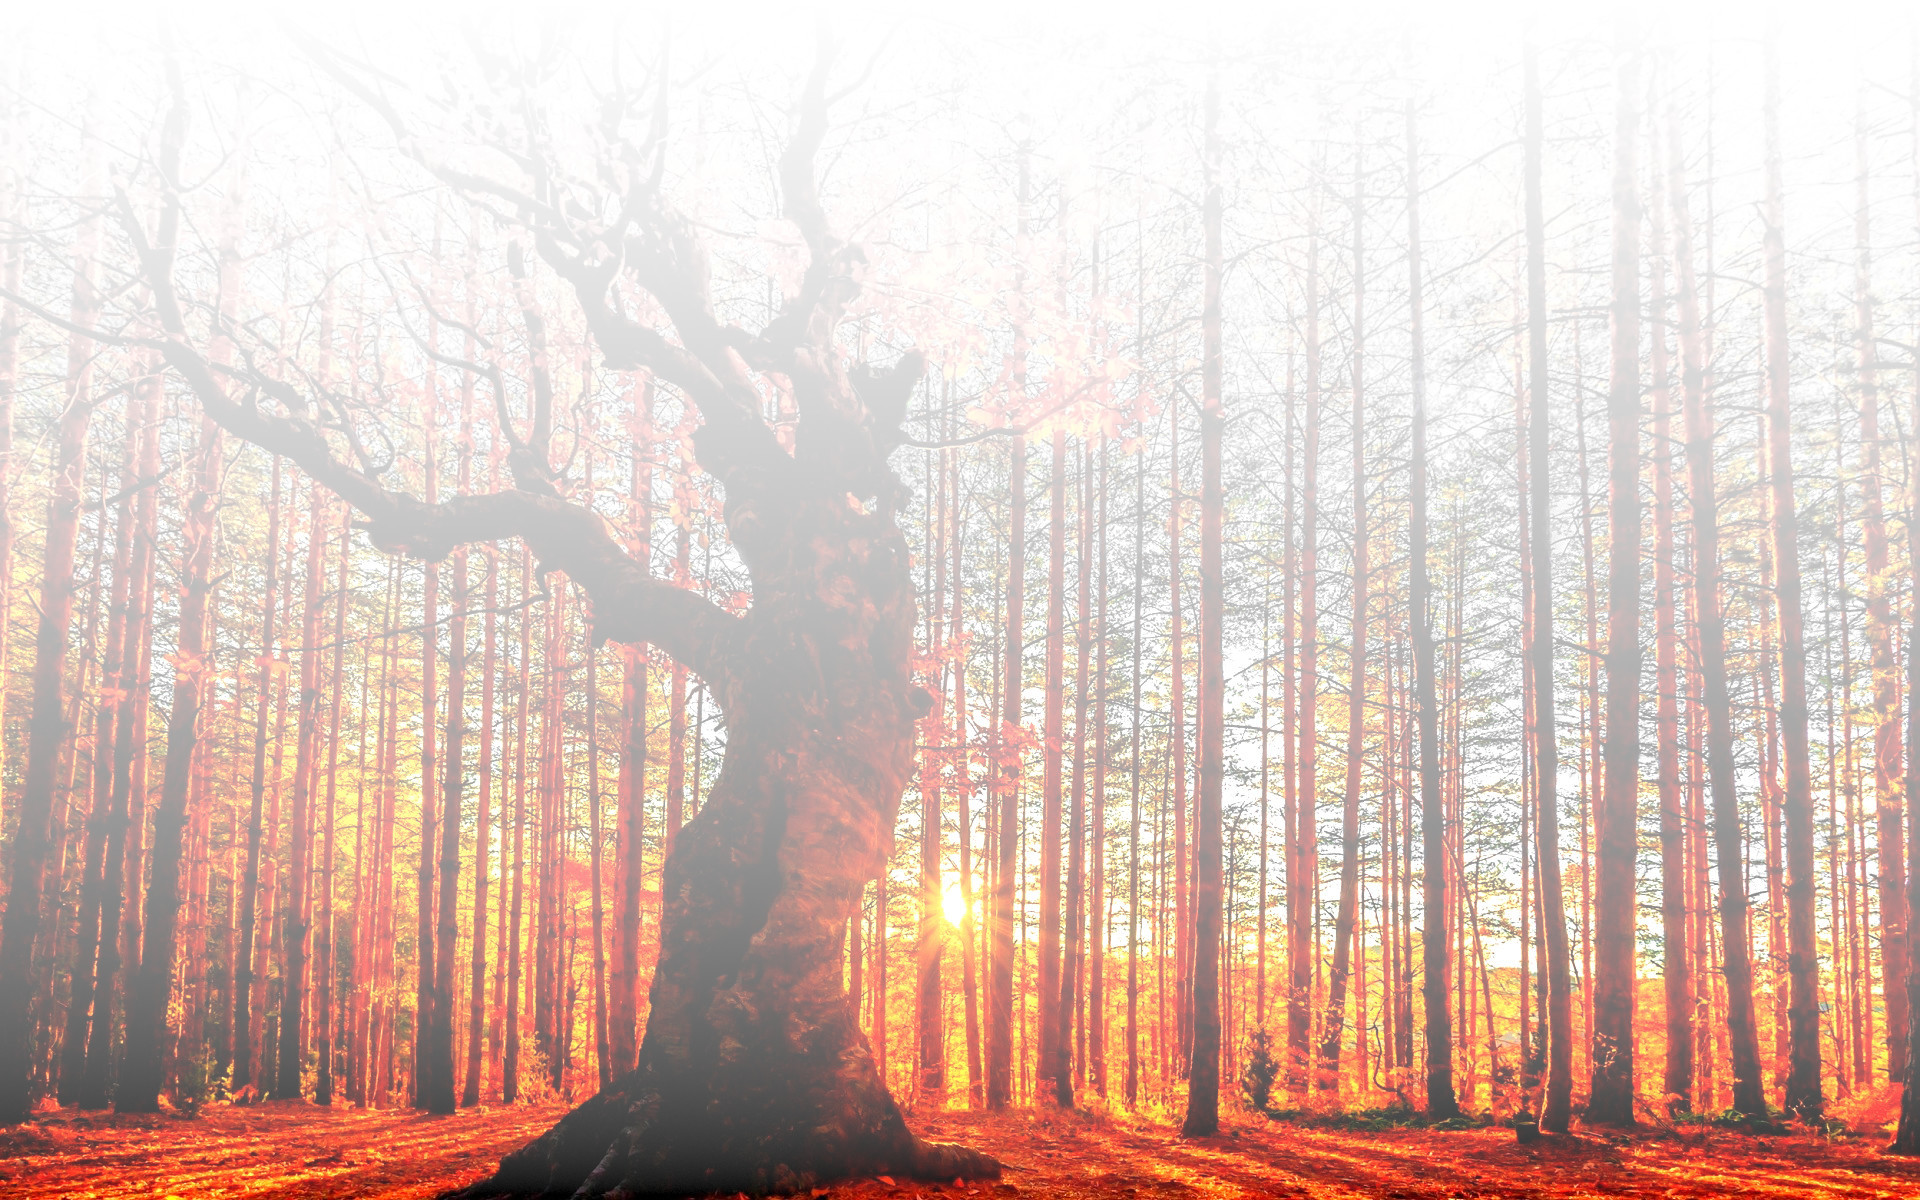
\includegraphics[width=\paperwidth]{forest-light}\end{minipage}}
\begin{frame}[c]
  \centering

  \bigskip
  %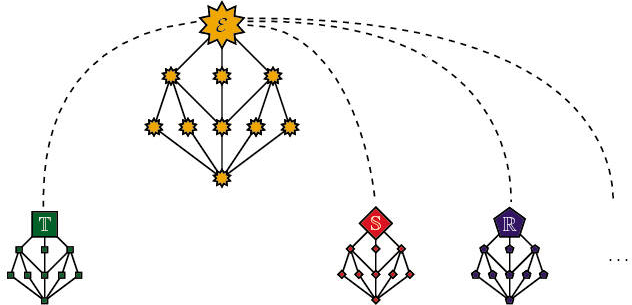
\includegraphics[height=0.32\textwidth]{olivia-lattices}
  \bigskip
  \bigskip
  \bigskip

  \scriptsize
  \textit{-- an invitation --}

  \setbeamercolor{block body}{bg=black!100}
  \begin{block}{}
  \centering\normalsize\color{white}
  Connecting \hil{inductive definitions},
  \hil{generic models} and \\ a \hil{modal multiverse} for algebra and combinatorics
  \end{block}

%  \begin{tikzpicture}
%    \def\R{8pt}
%    \node (title) {\vbox{\vspace*{-0.0em}Connecting \hil{inductive definitions},
%    \hil{generic models} and \\ a \hil{modal multiverse} for algebra and combinatorics
%    \\[0.8em]}};
%    \begin{pgfonlayer}{background}
%      \draw[decorate, very thick, draw=mypurple]
%        ($(title.south west) + (\R, 0)$) arc(270:180:\R) --
%        ($(title.north west) + (0, -\R)$) arc(180:90:\R) --
%        ($(title.north east) + (-\R, 0)$) arc(90:0:\R) --
%        ($(title.south east) + (0, \R)$) arc(0:-90:\R) --
%        cycle;
%    \end{pgfonlayer}
%  \end{tikzpicture}

  \bigskip
  \bigskip
  \bigskip
  \bigskip
  \bigskip
  \bigskip
  \bigskip

  REDCOM: \\
  \emph{Reducing complexity in algebra, logic, combinatorics} \\
  \ \\
  Brixen \\
  September 19th, 2022
  \bigskip

  Ingo Blechschmidt \\
  University of Augsburg
  \par
\end{frame}}

\definecolor{mypurple}{RGB}{150,0,255}
\setbeamercolor{structure}{fg=mypurple}


\section{Infinite data}

\begin{frame}{Infinite data}
  \vspace*{-0.6em}
  \begin{block}{}
    \justifying
    \textbf{Def.} A set~$X$ together with a binary relation~$R$ is
    \hil{almost-full$_\infty$} iff every \bad{\uwave{infinite sequence}}~$\alpha : \NN \to X$ is
    \hil{good} in that there exist numbers~$i < j$ such that~$\alpha(i)
    \mathrel{R} \alpha(j)$.
  \end{block}
  \vspace*{-0.6em}
  {\mbox{\small\emph{Examples.} $(\NN,{\leq})$,\ \ $X \times Y$ [Dickson],\ \
  $X^*$ [Higman],\ \ $\mathrm{Tree}(X)$ [Kruskal]} \\[-0.1em]
  \bad{Only classically.}
  \pause
  Constructive reformulation:
  \par}

  \begin{block}{}
    \justifying
    \textbf{Def.} For a predicate~$P$ on finite lists over~$X$, inductively
    define:
    \vspace*{-0.6em}
    \[
      \infer{P \,|\, \sigma}{P(\sigma)}
      \qquad
      \infer{P \,|\, \sigma}{\forall x \in X\_\ P \,|\, (\sigma :: x)}
    \]
  \end{block}
  \vspace*{-0.6em}
  {\small\justifying ``No matter how the finite approximation~$\sigma$ to an infinite
  sequence will \\[-0.1em] evolve to a better approximation, eventually~$P$ will hold.''\par}
  \pause

  \begin{block}{}
    \textbf{Def.} A set~$X$ together with a binary relation~$R$ is
    \hil{almost-full\textsubscript{ind}} iff~$\mathsf{Good} \,|\, []$, where
    $\mathsf{Good}(\sigma) \equiv (\exists i < j\_ \sigma[i] \mathrel{R}
    \sigma[j])$.
  \end{block}
  \vspace*{-0.8em}
  \begin{enumerate}
    \item Constructively, almost-full\textsubscript{ind} $\Rightarrow$
    almost-full$_\infty$. \vspace*{-0.2em}
    \item With \badbox{\textsc{lem}+\textsc{dc}}, almost-full\textsubscript{ind} $\Leftarrow$
    almost-full$_\infty$.
    %\pause
    %\item How much stronger is almost-full\textsubscript{ind}?
    %many-valued sequences, \ldots
  \end{enumerate}
\end{frame}


\section{Constructive red flags}

\begin{frame}{Constructive red flags}
  \vspace*{-0.5em}
  A transitive relation~$<$ on a set~$X$ is \ldots
  \begin{itemize}
    \item \ \\[-1.2em]\mbox{\hil{well-founded$_\infty$} iff
    there is no \bad{\uwave{infinite chain}} $x_0 > x_1 > \cdots$.}
    \item \hil{well-founded'$_\infty$} iff
    there is no \bad{\uwave{bad set}} (inhabited and such that for every member there is
    a smaller member).

    \item<4-> \hil{well-founded\textsubscript{ind}} iff for every~$x \in X$,
    $\mathsf{Acc}(x)$: %, where~$\mathsf{Acc}$ is inductively defined by:
    \[
      \infer{\mathsf{Acc}(x)}{\forall y < x\_\ \mathsf{Acc}(y)}
    \]
    \vspace*{-1.3em}
  \end{itemize}

  \pause
  \emph{Krull's Lemma:} An element~$x$ of a ring~$A$ is nilpotent if \ldots
  \begin{itemize}
    \item it is contained in
    every \bad{\uwave{prime ideal}}.
    \item<5-> the theory of prime ideals of~$A$ proves~``$x \in \ppp$''.
  \end{itemize}
  \medskip

  \pause
  \justifying
  \emph{Dependent choice:}
  Let~$R$ be a binary relation on a set~$X$
  such that~$\forall a \in X\_ \exists b \in X\_ a \mathrel{R} b$. Let~$x_0
  \in X$. Then there is an \bad{\uwave{infinite chain}} $x_0 \mathrel{R}
  x_1 \mathrel{R} x_2 \mathrel{R} \cdots$.
\end{frame}

%\begin{frame}{Inductive definitions}
%  \begin{block}{}
%    \justifying
%    \textbf{Def.} A transitive relation~$<$ on a set~$X$ is \hil{well-founded} iff
%    for all~$x \in X$, $\mathsf{Acc}(x)$, where the accessibility predicate is
%    inductively generated by:
%  \end{block}
%  \vspace*{-0.6em}
%  {\small\emph{Examples.} $(\NN,{<})$\par}
%
%  \textbf{Prop.} If~$<$ is well-founded, there are no infinite descending
%  chains~$x_0 > x_1 > \ldots$.
%
%  \emph{Proof.} By induction on~$x_0$.
%\end{frame}


\section{The set-theoretic multiverse}

{\usebackgroundtemplate{\begin{minipage}{\paperwidth}\vspace*{3.59cm}
\includegraphics[width=\paperwidth]{staircase}\end{minipage}}
\begin{frame}{The set-theoretic multiverse}
  \begin{tikzpicture}[remember picture,overlay]
    \node[xshift=-1.5cm,yshift=-4cm] at (current page.north east)
    {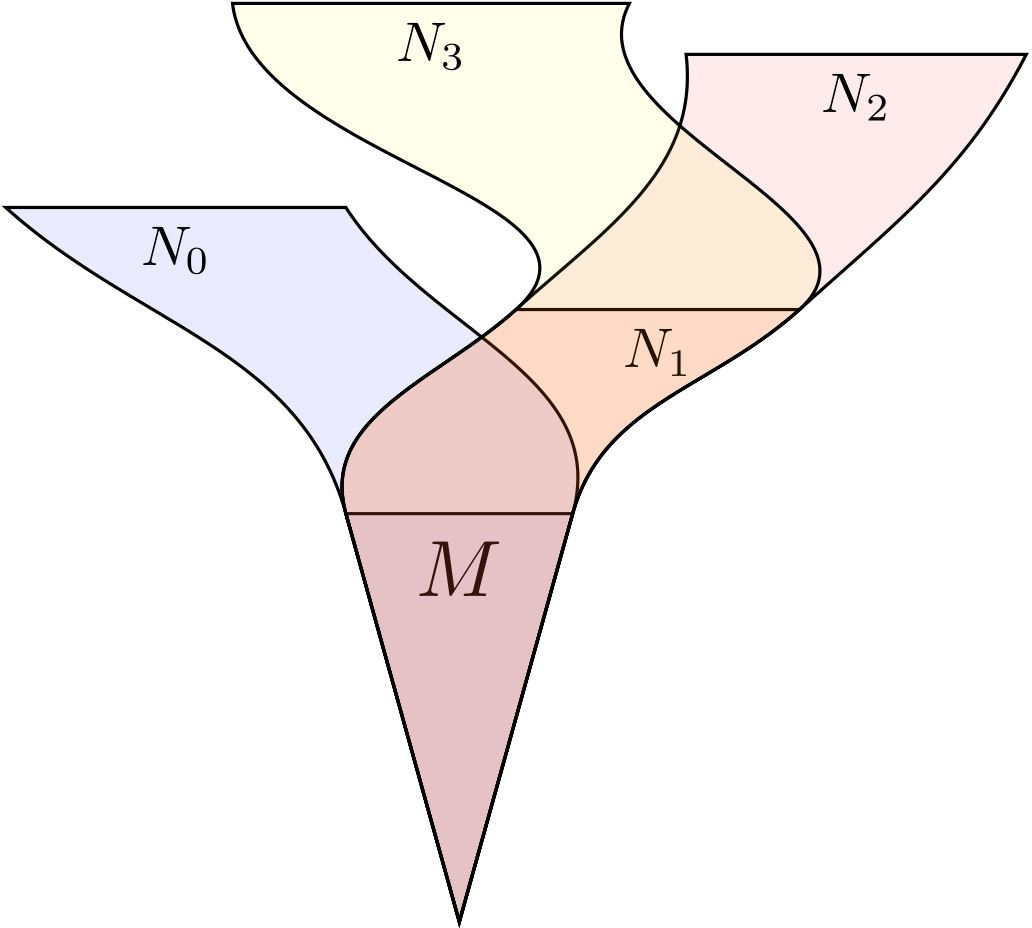
\includegraphics[width=2cm]{branching}};
  \end{tikzpicture}
  \vspace*{-2em}

  \begin{block}{}
    \justifying
    \textbf{Def.} A \hil{model of set theory} is a (perhaps class-sized) structure $(M,{\in})$
    satisfying axioms such as those of~\textsc{zfc}.
  \end{block}
  \vspace*{-0.6em}
  {\small\emph{Examples.}\vspace*{-0.8em}
  \begin{itemize}
    \item $V$, the class of all sets \vspace*{-0.6em}
    \item $L$, Gödel's constructible universe \vspace*{-0.6em}
    \item $V[G]$, a forcing extension containing a generic filter~$G$ of \\ some
    poset of forcing conditions \vspace*{-0.6em}
    \item Henkin/term models from consistency of (extensions of)~\textsc{zfc}
  \end{itemize}}
  \pause

  %{\centering\emph{Embracing all models of set theory:}\par}
  \begin{block}{}
    \justifying
    \textbf{Def.} $\possible\varphi$ iff~$\varphi$ holds in \hil{some extension} of
    the current universe. \\
    \phantom{\textbf{Def.}} $\necessary\varphi$ iff~$\varphi$ holds in \hil{all extensions}
    of the current universe.
  \end{block}
  \vspace*{-0.6em}
  \begin{itemize}
    \item $\necessary(\possible\textsc{CH} \wedge \possible\neg\text{CH})$,
    the continuum hypothesis is a \hil{switch}
    \item \ \\[-1.2em]\mbox{$\necessary\possible\necessary(\text{$X$ is countable})$,
    existence of an enumeration is a \hil{button}}
  \end{itemize}
\end{frame}}


\section{The topos-theoretic multiverse}

{\usebackgroundtemplate{\begin{minipage}{\paperwidth}\vspace*{5.95cm}
\includegraphics[width=\paperwidth]{fr1-lighter}\end{minipage}}
\begin{frame}{Toposes and generic models}
  \vspace*{-0.2em}
  \begin{changemargin}{-1.2em}{-1.2em}
  \begin{enumerate}
    \item\justifying A \hil{(Grothendieck) topos} is a category of sheaves over some
    \hil{site}.

    {\small\emph{Examples.} $\Set$, $\Sh(X)$, $\Set[\TT]$.\par}
    \bigskip
    \pause

    \item The \hil{Kripke--Joyal semantics} defines what it means for a
    statement~$\varphi$ to hold ``internally in a topos~$\E$'', written~``$\E
    \models \varphi$''. This semantics is sound with respect to intuitionistic
    logic.

%    {\small
%    \begin{itemize}
%    \item\justifying A statement holds in~$\Set$ iff it is true.
%    \item A statement holds in the ``topos of double-negation sheaves'' iff its
%    double-negation translation is true.
%    \item A statement holds in~$\Sh(X)$ iff a globalized version of it holds for
%    continuous families on the
%    space~$X$.\end{itemize}\par}
    \bigskip
    \pause

%    \item Every topos supports \hil{mathematical reasoning}: \\
%    If~$\ \E \models \varphi\ $ and if~$\ \varphi$ entails~$\psi$
%    intuitionistically,\, then~$\E \models \psi$.

    \item Let~$\TT$ be a geometric theory. The \hil{classifying
    topos}~$\Set[\TT]$ contains the \hil{generic~$\TT$-model}~$U_\TT$. It is
    \hil{conservative} in that for geometric implications~$\varphi$, the
    following are equivalent:
    \begin{enumerate}
      \item The statement~$\varphi$ holds for~$U_\TT$ in~$\Set[\TT]$.
      \item The statement~$\varphi$ holds for every~$\TT$-model in every
      topos.
      \item The statement~$\varphi$ is provable modulo~$\TT$.
    \end{enumerate}

    \begin{center}
      \begin{tikzpicture}[ultra thick, node distance=7mm]
        \node[rectangle, rounded corners=1pt, draw=lime!80, fill=lime!40] (a) {$\ZZ$};
        \node[rectangle, rounded corners=1pt, draw=lime!80, fill=lime!40, right=of a] (b) {$\ZZ[X,Y,Z]/(X^n+Y^n-Z^n)$};
        \node[regular polygon, regular polygon sides=5, draw=orange!80,
        fill=orange!20, right=of b, rounded corners=1pt, inner sep=0cm] (c) {$\O_X$};
        \node[star, rounded corners=1pt, star points=10, inner sep=0cm, draw=purple!80, fill=purple!20, right=of c] {$U_\TT$};
      \end{tikzpicture}
    \end{center}
  \end{enumerate}
  \end{changemargin}
\end{frame}}

\begin{frame}{Modal algebra and combinatorics}
  \begin{block}{}
    \justifying
    \textbf{Def.} A statement~$\varphi$ holds \ldots
    \begin{enumerate}
      \item\small \hil{everywhere} ($\necessary\varphi$) iff
      it holds in every (Grothendieck) topos (over the current base topos).
      \item \hil{somewhere} ($\possible\varphi$) iff
      it holds in some positive topos.
      \item \hil{proximally} ($\xpossible\varphi$) iff
      it holds in some positive ouvert topos.
    \end{enumerate}
  \end{block}
  \pause

  \newcommand{\seqbad}{\only<3>{infinite descending chain}\only<4->{bad set}}
  \begin{changemargin}{-2em}{-1.5em}
  \begin{enumerate}
  \small
    \item \justifying
    \only<1-4>{A relation is almost-full\textsubscript{ind} \\
    iff every infinite sequence \emph{everywhere} is good \\
    iff the \emph{generic infinite sequence} is good \\
    iff the \emph{theory of infinite sequences} proves goodness.\medskip}
    \only<5->{A relation is almost-full\textsubscript{ind} iff every infinite
    sequence \emph{everywhere} is good.}
    \pause

    \item\justifying
    \only<3-4>{A relation is well-founded\textsubscript{ind} \\
    iff \emph{everywhere} there are no \seqbad s \\
    iff the \emph{generic \seqbad} validates~$\bot$ \\
    iff the \emph{theory of \seqbad s} proves~$\bot$.}
    \only<5->{A relation is well-founded\textsubscript{ind} iff
    \emph{nowhere} there are \seqbad s.}
    \pause
    \pause
    \pause

    \item \only<2-6>{A ring element~$x$ is nilpotent \\
    iff \emph{everywhere} it is contained in all prime ideals \\
    iff it is contained in the \emph{generic prime ideal} \\
    iff the \emph{theory of prime ideals} proves~``$x \in \ppp$''.}
    \only<7->{\mbox{A ring element is nilpotent iff all prime
    ideals \emph{everywhere} contain it.}}

    \pause
    \pause
    \item Given an inhabited set~$X$, \emph{proximally} there is a surjection~$\NN
    \twoheadrightarrow X$ [J--T]. \\
    \hil{NB:} $(\possible\varphi) \Rightarrow \varphi$, if~$\varphi$ is a
    geometric implication. \\
    \phantom{\hil{NB:}} $(\xpossible\varphi) \Rightarrow \varphi$, if~$\varphi$
    is first-order. \\
    \phantom{\hil{NB:}} $\varphi \Rightarrow (\necessary\varphi)$,\, if~$\varphi$
    is a geometric formula.

    \pause
    \item Given~$(X,R,x_0)$ as in~\textsc{dc}, \emph{proximally} there is an
    infinite chain.

    \pause
    \item \emph{Somewhere,} the law of excluded middle holds. [Barr]
  \end{enumerate}
  \end{changemargin}
\end{frame}

{\usebackgroundtemplate{\begin{minipage}{\paperwidth}\vspace*{5.05cm}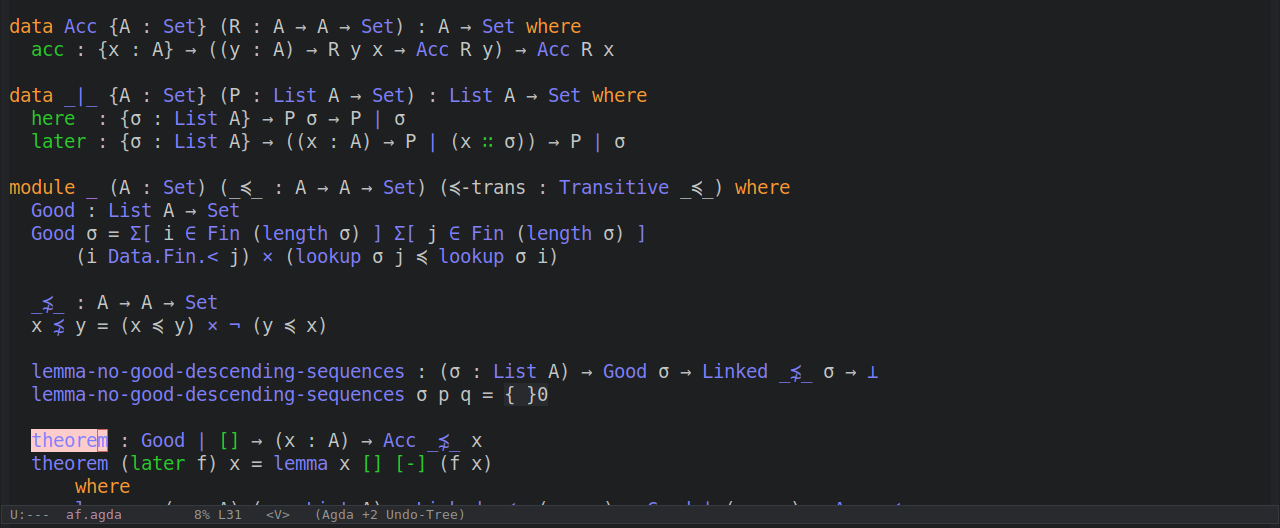
\includegraphics[width=\paperwidth]{agda-af-implies-wf}\end{minipage}}
\begin{frame}{Extracting constructive content}
  \begin{block}{}
    \justifying
    \textbf{Prop.} Let~$({\leq})$ be a transitive almost-full\textsubscript{ind} relation.
    Then~$({<})$, where~$x < y \equiv (x \leq y \wedge \neg(y \leq x))$,
    is well-founded\textsubscript{ind}.
  \end{block}
  \vspace*{-0.5em}

  \emph{Proof.} Everywhere, there can be no infinite descending chain, as any
  such would also be good. \qed

  \mbox{Unrolling this proof gives a program~$(\textsf{Good} \,|\, []) \to
  \prod_{x:X} \textsf{Acc}(x)$.}
  \vfill
\end{frame}}

\addtocounter{framenumber}{-1}
\begin{frame}{Extracting constructive content}
  \begin{block}{}
    \justifying
    \textbf{Thm.} [Dickson] If~$X$ and~$Y$ are almost-full\textsubscript{ind},
    so is~$X \times Y$.
  \end{block}
  \pause

  \vspace*{-0.3em}
  \emph{Proof.}\small
  \vspace*{-0.4em}
  \begin{enumerate}
    \item\justifying It suffices to verify that the \emph{generic infinite
    sequence}~$\gamma = (\alpha,\beta) : \NN \to X \times Y$ is good. \pause Since
    being good can be put as a geometric implication (in fact, a geometric
    formula) and since \textsc{lem} holds \emph{somewhere}, we may assume~\textsc{lem}.\pause

    \item By \textsc{lem} and well-foundedness, there is a minimal value~$\alpha(i_0)$
    among all values of~$\alpha$. \vspace*{-0.2em}\pause
    Similarly, there is a minimal value~$\alpha(i_1)$ among~$(\alpha(n))_{n >
    i_0}$, \pause a minimal value~$\alpha(i_2)$ among~$(\alpha(n))_{n > i_1}$, and so
    on. \pause By \emph{proximal dependent choice}, we can proximally collect these indices
    into a function~$i : \NN \to \NN$; this switches~\textsc{lem} off. \vspace*{-0.2em}\pause

    \item Switching~\textsc{lem} on again, there is a minimal value~$\beta(i(k_0))$
    among all values of~$\beta \circ i$. \pause Hence~$\gamma$ is good in view of
    \begin{align*}
      \alpha(i(k_0)) &\leq \alpha(i(k_0+1)), &
      \beta(i(k_0)) &\leq \beta(i(k_0+1)).
    \end{align*}
    \end{enumerate}
\end{frame}

% \begin{document}

{\usebackgroundtemplate{\begin{minipage}{\paperwidth}\vspace*{4.95cm}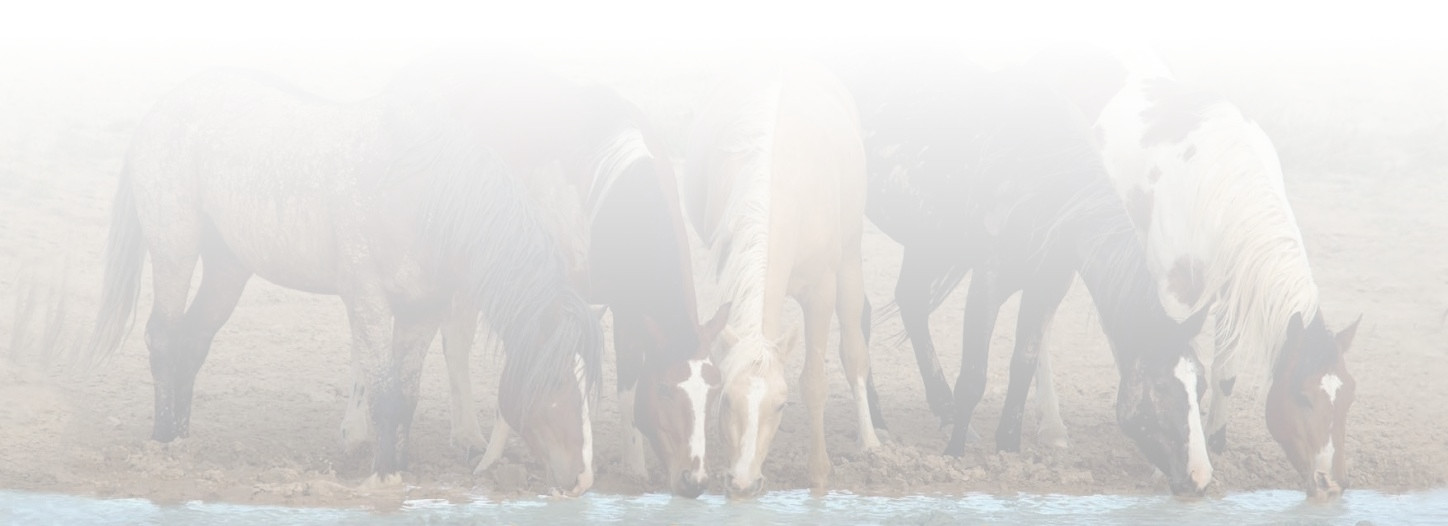
\includegraphics[width=\paperwidth]{topos-horses-lighter}\end{minipage}}
%{\usebackgroundtemplate{\begin{minipage}{\paperwidth}\vspace*{1.59cm}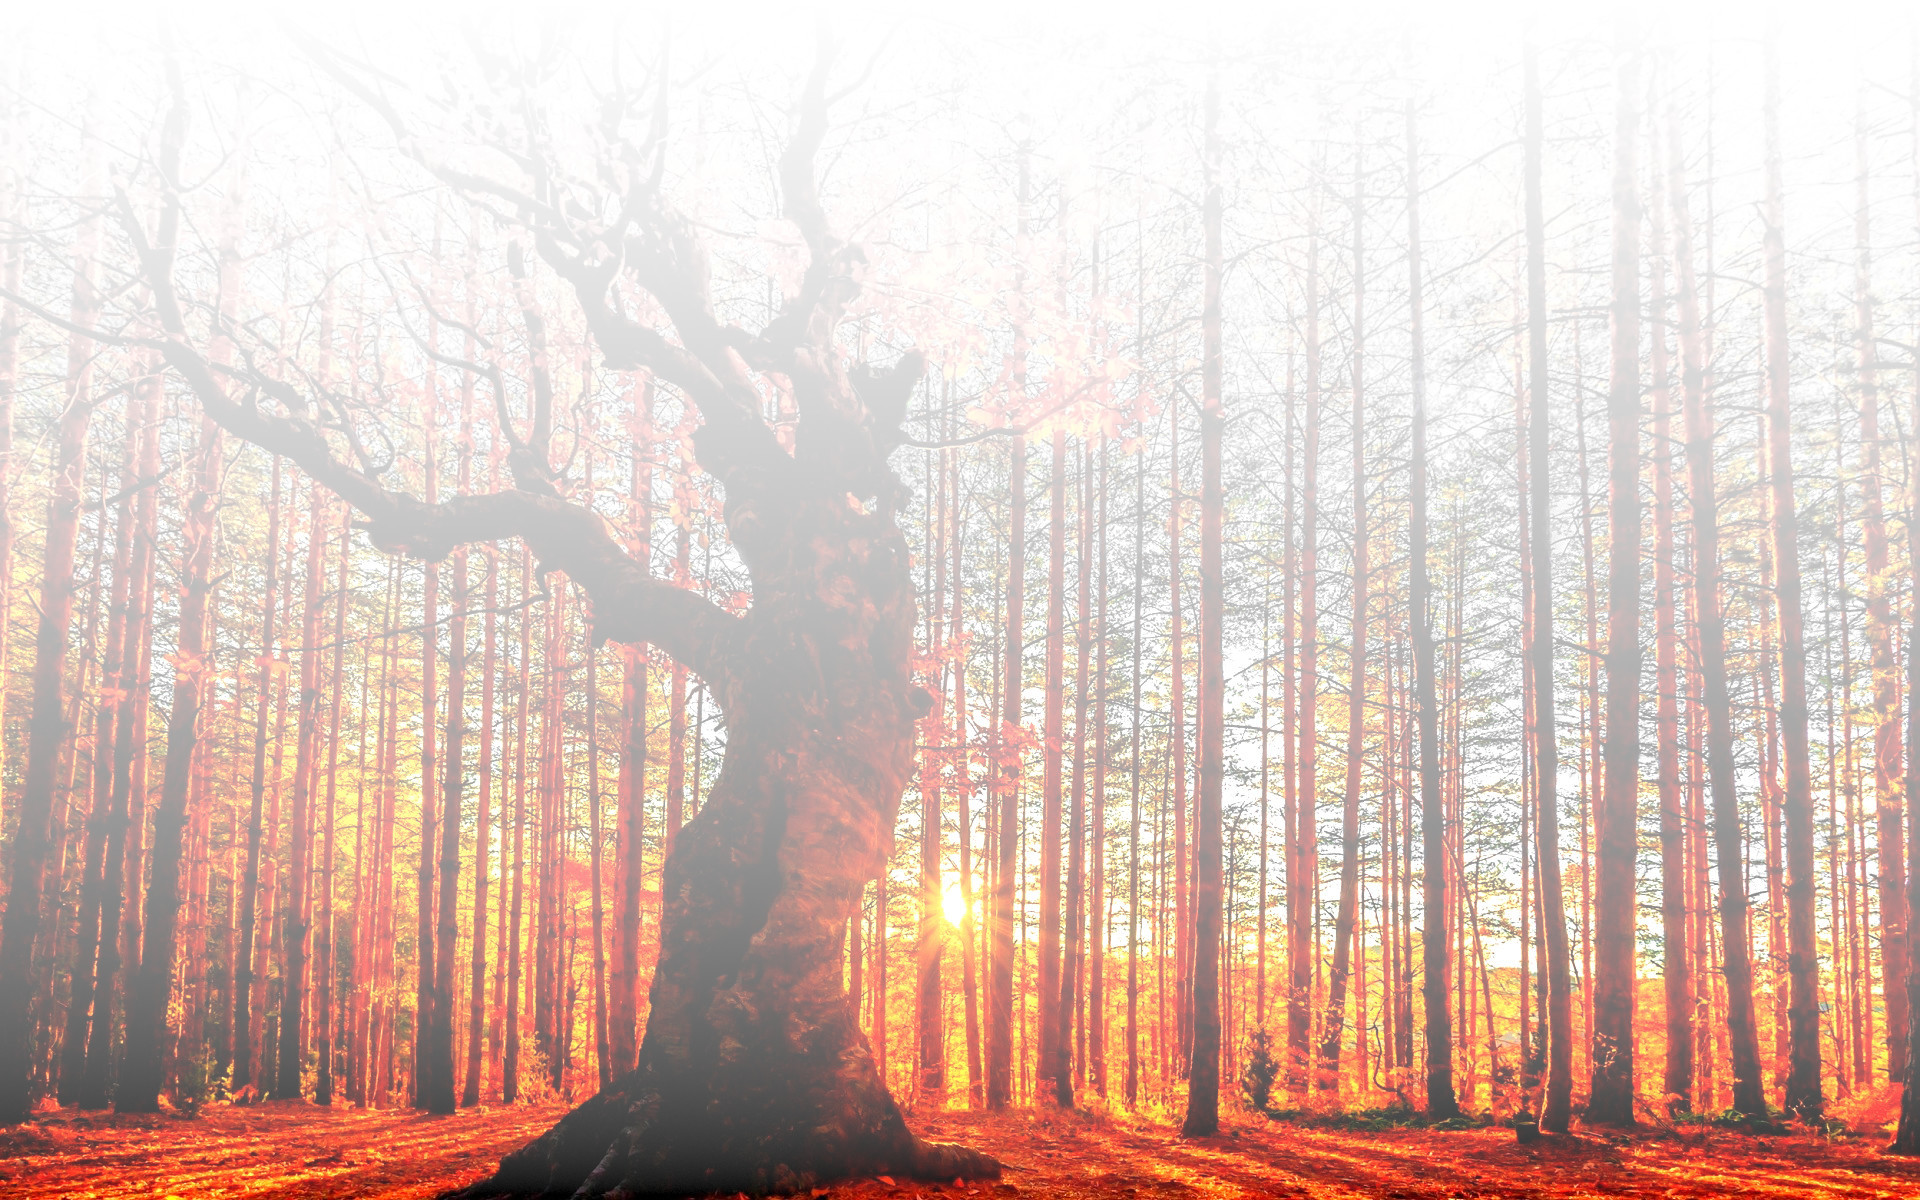
\includegraphics[width=\paperwidth]{forest-light}\end{minipage}}
\begin{frame}{Outlook}
  I learned the idea to study a modal multiverse of toposes from
  \hil{Alexander Oldenziel}, circa 2016. Foreshadowing results:
  \begin{itemize}
    \scriptsize
    \item[1984] André Joyal, Miles Tierney. \emph{An extension of the Galois theory of
    Grothendieck.}
    \item[1987] Andreas Blass. \emph{Well-ordering and induction in intuitionistic
    logic and topoi.}
    \item[2013] Shawn Henry. \emph{Classifying topoi and preservation of higher
    order logic by geometric morphisms.}
  \end{itemize}
  Work by Milly Maietti and Steve Vickers on \emph{arithmetic universes} is
  also closely connected. In progress:

  \begin{itemize}
    \item Develop details and formalize.
    \item Determine the precise list of valid modal principles.
    \item Carry out case studies with program extraction.
    \item Incorporate the right adjoints of geometric morphisms.
  \end{itemize}
\end{frame}}

\addtocounter{framenumber}{-1}

\end{document}

Choice:
erst abzählbar machen,
dann DC
nein, funktioniert nicht ganz
aber für diskrete Quelle habe surjektive (nicht offene?) Theorie/Topos

∀x ∈ X. ∃y ∈ Y. φ(x,y).
(Toposwechsel für Abzählbarkeit von X)
∀n ∈ ℕ. ∃y ∈ Y. φ(πn,y).
Yn := { y ∈ Y | φ(πn,y) }
(~) auf M = (coprod_n Y_n): (n,y) ~ (n',y') gdw. n' = n+1
Dann habe: M bewohnt (durch (0,...)) und ∀p ∈ M. ∃q ∈ M. p ~ q.
(Toposwechsel für DC für (~))
Habe f : ℕ → M mit f(0) = (0,...) und f(n) ~ f(n+1) für alle n.
Also ist π₂.f eine Auswahlfunktion, genauer: ∀n. φ(πn, π₂(f(n))).

Zorn für abzählbare Mengen?
C_0 = {}
C_{n+1} = C_n cup { x_n | C_n cup {x_n} Kette }
C = bigcup_n C_n
z = sup(C)
Dann ist z maximal?
Gelte z ≤ e.
Dann ist C cup { e } Kette.
Wenn e = x_n0, so insbesondere C_n0 cup { e } Kette.
Also e ∈ C_{n+1} ⊆ C, also e ≤ z.
Also e = z.
Problem: Kommt eher selten vor; Supremum wird oft nicht zur Menge gehören.
Beispiel: Supremum von Menge endlich erzeugter Ideale ist nicht endlich erzeugt.

0: title
* expectations: no new method for extracting constructive content, rather
  point of view for putting previous work in a uniform context;
  philosophy turned mathematics

1: infinite data
* how much more general? multivalued sequences, "¬¬ sequences", ...
* where do these definitions come from? conceptual answer

3: set-theoretic multiverse
* axioms of ZFC massively underspecify the concept of sets;
  models for exploring the range of set-theoretic possibility
* to settle a question shown to be independent from ZFC is to
  understand how it behaves in the multiverse

4: topos and generic models
* truth in Set, truth in double-negation sheaves, truth in Sh(X)
* generic ring, generic group, ...
